%!TEX root = thesis.tex

\renewcommand{\TheTitle}{Influence of Wind on Flaming Ignition of Porous Wood Fuel Beds}
\renewcommand{\TheAuthors}{Derek Bean, David L. Blunck}

\renewcommand{\TheAddress}{
\textbf{Status: In Preparation}
}

\PaperHeader{\TheTitle}{\TheAuthors}{\TheAddress}

\chapter{\TheTitle}
\label{part:manuscript2}

\section{Abstract}
    The increasing severity of wildfires and the expansion of the wildland urban interface has increased the need to better protect homes from fires. Ignition of fuels (e.g., needles, mulch, leaves) near or on homes by firebrands can be a significant risk factor for home loss. Understanding the environmental factors that control the ignition of fuel beds by firebrands is important to reducing the risk of home loss. This study evaluates the effect of the wind speed and direction on the probability of ignition of fuel beds by firebrands. The fuel beds, Douglas-fir particles between 1.3\si{\milli\meter} and 2.3\si{\milli\meter} in size, were ignited by a cartridge heater (i.e., surrogate firebrand). Flaming ignition probability and time to ignition were determined for three different wind speeds and three wind directions. CFD calculations were performed to provide additional insights into the flow field leading up to ignition. Increases in wind speed above quiescent conditions reduced the temperature required for flaming ignition. An increase in wind speed to 3.5\si{\meter\per\second} from quiescent increased the ignition probability of fuel beds from 60\% to roughly 100\% depending on the wind direction. However, a threshold was observed for some wind directions where a further increase of wind did not increase the ignition probability. Temperatures required for flaming ignition and the time to ignition were sensitive to the wind direction. Ignitions occurred at the lowest temperatures when the wind direction was perpendicular to the surrogate firebrand. High speed images of the ignition process and  corresponding CFD calculations indicate that ignition occurred in regions with long residence times. The sensitivity to wind direction is attributed to differences in recirculation zones which changes the residence time of pyrolyzates. 
    
\section{Introduction} 

    As the severity of wildfires and the number of homes in the wildland urban interface (WUI) increases the need is rising to better protect homes from wildfires~\cite{Marlon2012Long-termUSA, Manzello2013, Barrett2020}. A common way that homes are destroyed during wildfires is by the ignition of fuel beds (e.g., needles, leaves, or landscaping materials) by firebrands. Flames may then spread to and subsequently engulf the structure~\cite{Manzello2014, Maranghides2011AFires}. A better understanding of how fuel beds ignite around homes is necessary in order to better protect homes from this phenomena. While the overall mechanisms by which ignition by firebrands occur are generally well understood, predicting when ignition will occur remains elusive~\cite{Fernandez-Pello2017}. One of the reasons for the limitations of predictive capabilities is the lack of quantification with respect to how changes in the fuel bed and environmental conditions influence the likelihood of ignition~\cite{Finney2013}.
    
    Wind is an environmental factor that can have a significant impact on the spread of fires. First, increases in wind speed increase the size of firebrands produced~\cite{Suzuki2013}, potentially leading to firebrands of higher energy content. Second, firebrand laden winds flowing around structures can lead to accumulation of firebrands in particular regions~\cite{Suzuki2020a, Manzello2014}. Third, the amount of heat imparted to a fuel bed by firebrands can increase as wind speeds increase~\cite{Hakes2019a, Tao2020, Salehizadeh2021}. 
    
    In many studies the presence of wind either increases the probability of ignition by firebrands~\cite{Filkov2016, Manzello2006, Manzello2006a, Matvienko2018, Ellis2015, Plucinski2008}, or facilitated ignitions that did not occur without wind~\cite{Ellis2011}. For example, in tests with natural fuel beds (e.g, needles, leaves, and grass) and firebrands (e.g., burning twigs, bark, and cones) increases in ignition probability were observed, in some instances, with increases in wind speeds and changes in wind direction~\cite{Ganteaume2009}. Similar increases in ignition probability as wind speed increases have been observed in fuel beds with hot metal particles as ignition sources~\cite{Wang2017}. Increases in ignition propensity have been postulated to be caused by greater oxygen availability and/or increased mixing as a result of the wind speed. 
    
    In the aforementioned studies the heat transfer rates from the firebrands to the fuel beds may have changed (likely increased due of faster reaction rates) due to the presence of wind. Changes in the heat transfer rate from the firebrands and changes in the flow field near the fuel bed make it challenging to fully identify cause(s) for wind increasing/altering ignition behavior.
    As a result it is not clear to what extend changes in ignition behavior are caused by the interaction of the fuel bed with the wind or changes in heat transfer from the firebrands.
    It is important to decouple these two effects to better understand how each factor impacts ignition. A better understanding of ignition sensitivities to wind can ultimately be used to better design building codes and standards to protect structures near the WUI.

    
    
    %A similar increase in ignition propensity in the presence of wind has been observed for fuel beds in contact with hot metal particles, in contrast to firebrands~\cite{Wang2017}. This observations suggests that a sensitivity to oxygen availability caused by wind over the fuel bed independent from the effects of heat transfer from firebrands due to wind. Ultimately, the magnitude of the impact that increasing mixing and oxygen availability has on ignition of fuel beds has not been isolated or characterized with respect to wildland fire applications. Such knowledge can be used to ensure that models and/or test standards capture the required physics.
    
    %Fortunately, a framework for considering the relative effects of mixing and oxygen availability exists. This relationship is the Damkohler number (Da)\cite{Law2006CombustionPhysics}. The Da is typically used to predict ignition of gaseous fuel-oxidizer mixtures relative to the ratio the the fluid dynamic residence time and the time for chemical reactions to occur. 
    
    With this background and motivation, the objective of this study is to quantify how changing environmental factors, specifically wind speed and direction, influences ignition of a fuel bed in contact with a firebrand. It is expected that the results of this work will help further the understanding of the influence of wind on fuel bed ignition and may allow for better protection of structures in the WUI.

\section{Methodology}

    The probability of flaming ignition for beds of Douglas-fir particles were measured for three different wind speeds and firebrand orientations in a wind tunnel. Douglas-fir particles serve as a surrogate for natural fuels near the WUI. Figure~\ref{fig:windTunnelApparatus} shows a representation of the wind tunnel, fuel bed, and the portion of the device for lowing a cartridge heater (i.e., surrogate firebrand) onto the fuel bed.  The wind speeds tested were 0.5 \si{\meter\per\second}, 3.5 \si{\meter\per\second}, and 5.8 \si{\meter\per\second}. Higher wind speeds were not tested to avoid material from the fuel bed blowing away. The wind speed was measured with a TSI-IFA300 hot wire probe. Tests were conducted with the heater placed parallel, perpendicular, and 45\si{\degree} relative to the wind direction for each wind speed. 

    
    The fuel beds were created in a multi-step process. Kiln dried Douglas-fir lumber was planed, then granulated, and finally screened such that the particles fit through a 2.3\si{\milli\meter} screen but not a 1.3\si{\milli\meter} screen. The fuel was placed in a 140\si{\milli\meter} diameter glass container with a depth of 70\si{\milli\meter} before insertion into the wind tunnel. The average bulk density of the fuel beds was 74.2\si{\kilo\gram\per\cubic\meter}.   
    
    A minimum of 20 ignition tests were conducted for each experimental condition with a total of 241 tests.  The temperature set points of the heater for the various experiments were identified using the three-phase optimal design procedure~\cite{Wu2014, Burke2017TestPractice}. The three-phase optimal design is a sequential procedure used to ascertain the probability of a binary outcome (i.e., ignition or non-ignition) with a limited number of tests. The logistic regressions and 95\% confidence intervals of the ignition probability were calculated using the scikit-learn python package~\cite{scikit-learn}. A fuel bed was considered to ignite if a flame was observed and persisted after the heater was removed. If flaming ignition was not observed after 3000\si{\second} of heater contact the heater was removed and the test was considered to have a no-ignition outcome.
     \begin{figure}[hbpt]
            \centering
            \resizebox{0.5\columnwidth}{!}{%
                \begin{tikzpicture}
                    \filldraw[pattern=north west lines, pattern color=brown, thick] (2.84, 0)  rectangle (4.34, -.75) node[pos=0.5,rectangle,fill=white] {\scriptsize Fuel Bed};
                    \fill [draw=white,  inner color=red, outer color=white ] (3.59, 0.01) circle (0.15);
                    \filldraw[draw=black,fill=white, thick] (0, 0)      rectangle (6, 3);
                    \fill[fill=black!50] (3.58, 0) rectangle (3.61, 1.52);
                    \fill[fill=black] (3.55, 1.52) rectangle (4.23, 1.57);
                    \filldraw[draw=black, fill=black!50] (4.09, 1.57) rectangle (4.22, 3);
                    \fill[draw=red, fill=red] (3.59, 0.01) circle (0.0635);
                    \draw [<-] (3.5, 0.1) -- (3, 0.5) node[left] {\scriptsize Heater};
                    \draw [<-] (3.5, 1.55) -- (3, 1.55) node[left] {\scriptsize Load Cell};
                    \draw [<-] (3.75, 2.5) -- (3, 2.5) node[left] {\scriptsize Lowering Arm};
                    \draw[->]         (0.1, 0.6) -- (0.75, 0.6);
                    \draw[->]         (0.1, 1.2) -- (0.75, 1.2);
                    \node[right] at (-0.75, 1.5) {\scriptsize Inlet};
                    \draw[->]         (0.1, 1.8) -- (0.75, 1.8);
                    \draw[->]         (0.1, 2.4) -- (0.75, 2.4);
                    \draw[draw=black, dashed] (3.336, 0) rectangle (4.54, 0.34);
                    \draw[->]         (4.3, 1) -- (4.0, 0.34);
                    \node[right, align=left] at (4.3, 1) {\scriptsize Computational\\ \scriptsize Domain};
                \end{tikzpicture}
                }
            \caption{Diagram of the experimental wind tunnel apparatus. Air flows through the wind tunnel from left to right. The dashed region represents the domain subset used for computational efforts.}
            \label{fig:windTunnelApparatus}
        \end{figure}
    
    The energy imparted to the fuel bed was estimated by applying an energy balance to the heater. Typical heat fluxes to the fuel bed ranged from 5\si{\kilo\watt\per\square\meter} to 50\si{\kilo\watt\per\square\meter}. Similar values have been reported for studies of heat fluxes from firebrands~\cite{Hakes2019a, Tao2020}. The power delivered to the heater was measured using a CR9580-10 current sensor and a ZMPT101B voltage sensor. Temperature distributions, created from infrared images of the heater taken with a FLIR SC6700 camera, were used to estimate heat loss to the ambient. A black body calibration was performed to correlate photon counts from the camera to temperature and produce a longitudinal temperature distribution. The circumferential temperature of the heater was considered uniform.
    
    High speed images of the ignition process were captured using a Phantom VEO 710 camera for select conditions. The images were used to provide insights into differences between ignition processes. Images were collected at 5\si{\kilo\hertz}. 
    
    A simplified computational model was implemented to provide further insights into the processes leading up to ignition for the different configurations. Fluid flow around the heater, heat transfer from the heater to the fluid, and the release of pyrolysis gases into the fluid domain were simulated for the 5.8\si{\meter\per\second} wind speed and the three heater orientations. Simulations were conducted in two parts. First the average mass flux and average thermal properties of pyrolyzates were estimated. These estimations were conducted through a non-reacting heat transfer model to the fuel bed to obtain an estimate for the mass of fuel bed material above the pyrolysis temperature of 220\si{\celsius}. The thermal properties of the fuel bed were estimated using correlations for porous media~\cite{bergman2011fundamentals} and the average bulk density of the fuel beds during the tests. The heat transfer to the fuel bed was determined from the energy balance for a heater temperature corresponding to the 50\% ignition probability. The mass of pyrolysis gases released was then estimated using 0D calculations in Cantera. The chemical composition of the fuel bed was estimated from the Bioengineering Feedstock Library database~\cite{feedstock}. The BioPox mechanism~\cite{Dhahak2019} was used for pyrolysis kinetics in the fuel bed. Species were considered to be released into the flow domain if they existed in the gas phase biomass mechanism Bio1412~\cite{Ranzi2008}. More detail for the species selection process is available in previous work~\cite{Bean2021}.
    
   The second step of the computational effort simulated pyrolysis gas distribution in near the heater using OpenFOAM~\cite{Foundation2020}. The computational domain used is outlined in Figure~\ref{fig:windTunnelApparatus} with a dashed rectangle. The local equivalence ratio was calculated after one second of pyrolysis release. While these times are much less than the average time to ignition, insights are still gained into the distribution of pyrolyzates with respect to the observed ignition locations for the heater orientations.
    
\section{Results and Discussion}
    The ignition or no ignition outcomes of the the tests are shown in Figure~\ref{fig:heaterAngle}. Individual markers in the plots represent the outcome of each test. The curves are logistic regressions for each of the test groups (i.e., tests with the same wind speed and heater angle) with shaded regions around the curves indicating the 95\% confidence interval of the regressions. The tests are grouped such that each plot shows tests of different wind speeds at the same heater orientation. The topmost plot shows results when the heater is parallel to the flow, the middle plot when the heater is 45\si{\degree} to the flow, and the bottom plot when the heater is perpendicular to the flow. 
        \begin{figure}[hpbt]
            \centering
            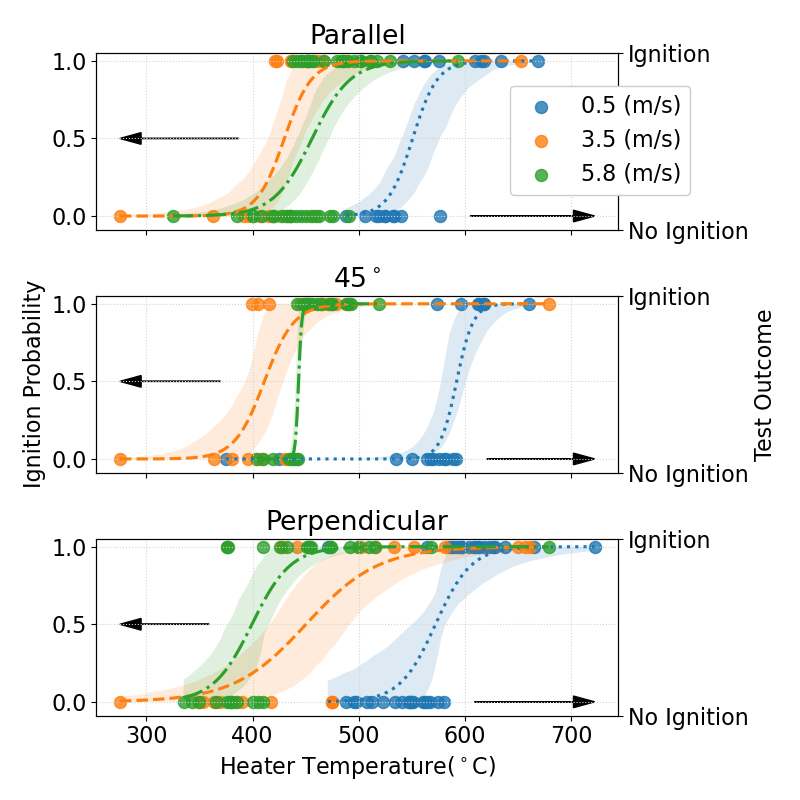
\includegraphics[width=0.5\columnwidth]{Figures/heat_angle_hist_names.png}
            \caption{Ignition or no ignition outcomes of tests at different bulk wind speeds with respect to heater orientation. Markers indicate the outcome of each test and the curves show the logistic regression of each test group. The shaded regions show 95\% confidence intervals for each regression.}
            \label{fig:heaterAngle}
        \end{figure}
    The three different sets of data in each plot are the results for the experiments with three wind speeds. Table~\ref{tab:fiftyTemp} shows the heater temperatures estimated to produce a 50\% ignition probability for the results shown in Figure~\ref{fig:heaterAngle}.
        \rowcolors{2}{gray!25}{white}
            \begin{table}[hpbt]
                \normalsize
                \caption{Heater temperature required to achieve 50\% ignition probability for the wind speeds and heater angles tested.}
                \centering
                \begin{tabular}{crrr}
                    \rowcolor{gray!50}
                   U\textsubscript{bulk} (\si{\meter\per\second}) & 0 \si{\degree} (\si{\celsius}) & 45\si{\degree} (\si{\celsius}) & 90\si{\degree} (\si{\celsius})\\
                    \hline
                    0.5  & 551 & 592 & 571\\
                    3.5  & 430 & 411 & 450\\
                    5.8  & 456 & 443 & 399
                \end{tabular}
                \label{tab:fiftyTemp}
            \end{table}
    Three observations are noted for the results in Figure~\ref{fig:heaterAngle} and Table~\ref{tab:fiftyTemp}. 
    First, the ignition probability for the 0.5\si{\meter\per\second} cases are similar to previously published results for a similar fuel bed and apparatus with measured wind speeds of 0.1\si{\meter\per\second}\cite{Bean2021}. Second, increasing the wind speed beyond 0.5\si{\meter\per\second} increased the ignition probability. This observation is consistent with previously reported work~\cite{Ganteaume2009, Matvienko2018} that showed that the presence of wind can increase the likelihood of ignition. What has not been quantified previously is the magnitude of the difference in ignition probability due to wind speed. For example, in tests with the heater oriented parallel to the flow, a heater temperature expected to produce ignition 25\% of the time at a wind speed of 0.5\si{\meter\per\second} is anticipated to produce ignitions for greater than 99\% of tests at 3.5\si{\meter\per\second} and 5.8\si{\meter\per\second}. The difference is even more pronounced for the 45\si{\degree} and perpendicular orientations where heater temperatures expected to result in ignition less than 1\% of tests at 0.5\si{\meter\per\second} have an ignition probability of over 99\% at 5.8\si{\meter\per\second}. This observation illustrates that an increase in wind speed that is relatively modest (compared to winds often accompanying wildfires) can shift fuel bed ignition risk from minimal to very likely with no other changes in conditions.
    
    The third observation from Figure~\ref{fig:heaterAngle} and Table~\ref{tab:fiftyTemp} is that while an increase in wind speed from 0.5\si{\meter\per\second} to 3.5\si{\meter\per\second} resulted in an increase in ignition probability for all heater angles, an increase from 3.5\si{\meter\per\second} to 5.8\si{\meter\per\second} does not. For tests where the heater was perpendicular to the flow (90\si{\degree}) an increase in wind speed led to a decrease in heater temperatures required for ignition. For tests with the heater at 45\si{\degree} to the oncoming flow, ignitions were observed at the lowest temperatures in the 3.5\si{\meter\per\second} case. For the parallel heater case the difference in ignition between the 3.5\si{\meter\per\second}, and 5.8\si{\meter\per\second} cases were not statistically significant. These trends in ignition propensity suggest that there is a threshold for ignition enhancement that depends on both wind speed and orientation of the wind with respect to the firebrand. A threshold for an optimum wind speed for inducing ignition has been postulated~\cite{Plucinski2008} but this is one of the first studies to confirm its existence and dependence on the orientation of the wind.
    
    Figure~\ref{fig:windSpeed} shows the data reported in Figure~\ref{fig:heaterAngle} but organized to more easily highlight sensitivities of ignition behavior for the different heater angles for a constant wind speed. Three observations are noted. First, differences in ignition probability were not statistically significant for the various heater orientations and a wind speed of 0.5\si{\meter\per\second}. This suggests, as anticipated, that for near quiescent conditions the orientation of the firebrand is less important than the temperature of the firebrand. Second, for the 3.5\si{\meter\per\second} tests there was not a statistically significant difference in ignition temperatures for the parallel and 45\si{\degree} heater orientations, but there is a statistically significant difference at the 5.8 \si{\meter\per\second} case. The differences in sensitivities between the two wind speeds is attributed to the lowest temperature required for ignition (maximum ignition enhancement) occurring for a wind speed of 3.5\si{\meter\per\second} for the 45\si{\degree} orientation. The maximum enhancement of ignition for the perpendicular case appears to occur at a wind speed above 3.5\si{\meter\per\second}. The third observation is that changing the angle of the heater relative to the wind direction has less of an influence on ignition behavior than changing the wind speed.
    Thus, for a fixed heater temperature, an increase in wind speed will yield a larger increase in ignition probability when compared to changing the firebrand orientation. This is only true, however, up to the wind speed that produces the greatest likelihood of ignition. 
    
    At and above the wind speed that produces the greatest likelihood of ignition for a given firebrand orientation, an increase in ignition will only occur if the angle between the firebrand and wind is increased to become more perpendicular to the flow. 
    The aforementioned observations affirm that both the wind speed and direction can alter the likelihood of flaming ignition of a fuel bed. What is unclear, thus far, are the specific physical processes that promote or retard ignition as the wind speed is increased or the heater angle is changed.  
    
        \begin{figure}[hpbt]
            \centering
            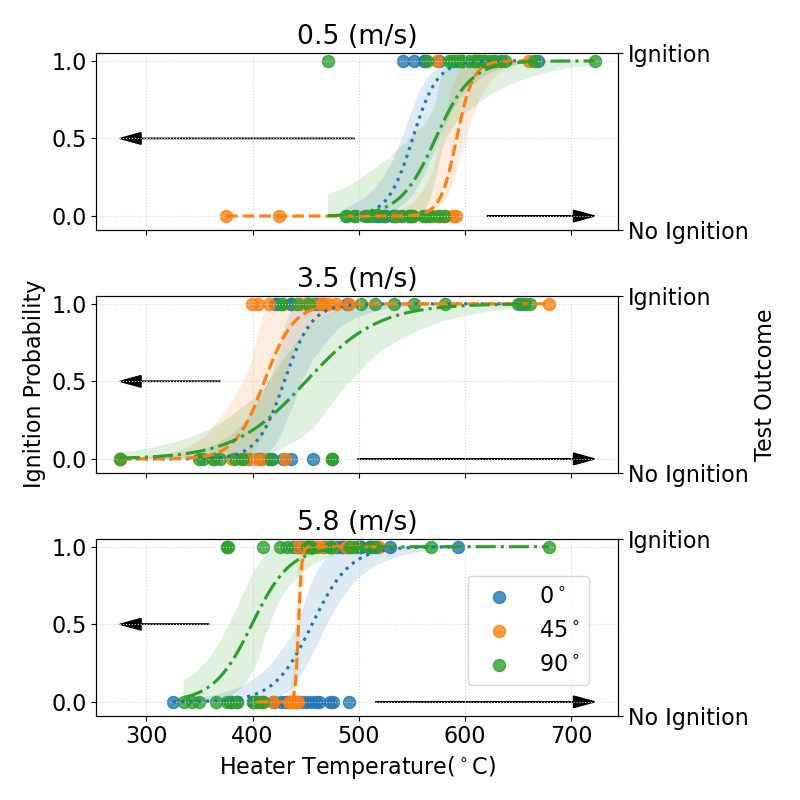
\includegraphics[width=0.5\columnwidth]{Figures/stacked_wind_speed.png}
            \caption{Ignition or no ignition outcomes of tests at different heater angles with respect to wind speed. Markers indicate the outcome of each test and the curves show the logistic regression of each test group. The shaded regions show 95\% confidence intervals for each regression.}
            \label{fig:windSpeed}
        \end{figure}
    
    In contrast to the observed sensitivities of wind speed on ignition probability the time to ignition is more sensitive to the heater orientation than the wind speed. Figure~\ref{fig:histogramFigure} shows histograms of the time to ignition (i.e., occurrence of flames) for each test where ignition was observed. The wind speed increases from the top plot to the bottom plot and the color of each group in the plot represents the different heater angles. Note that the time to ignition axis is log-scale. Three observations are noted about the time to flaming ignition. First, the times to ignition for the 3.5\si{\meter\per\second}, and 5.8\si{\meter\per\second} wind speeds often are sufficiently long (i.e., \textgreater 100\si{\second}) enough to suggest that the fuel beds may be igniting in a smoldering mode and then transition to flaming. Second, for the 0.5\si{\meter\per\second} tests the difference in time to ignition between the heater angles are much smaller than for the other two wind speeds. Third, for the 3.5\si{\meter\per\second}, and 5.8\si{\meter\per\second} cases ignition times are typically longest when the heater is oriented parallel to the flow. The shortest times to ignition typically occurred when the heater was perpendicular to the flow. The sensitivity of time to ignition to different heater angles suggests that the ignition process changes as the heater angle changes.
        \begin{figure}[hpbt]
            \centering
            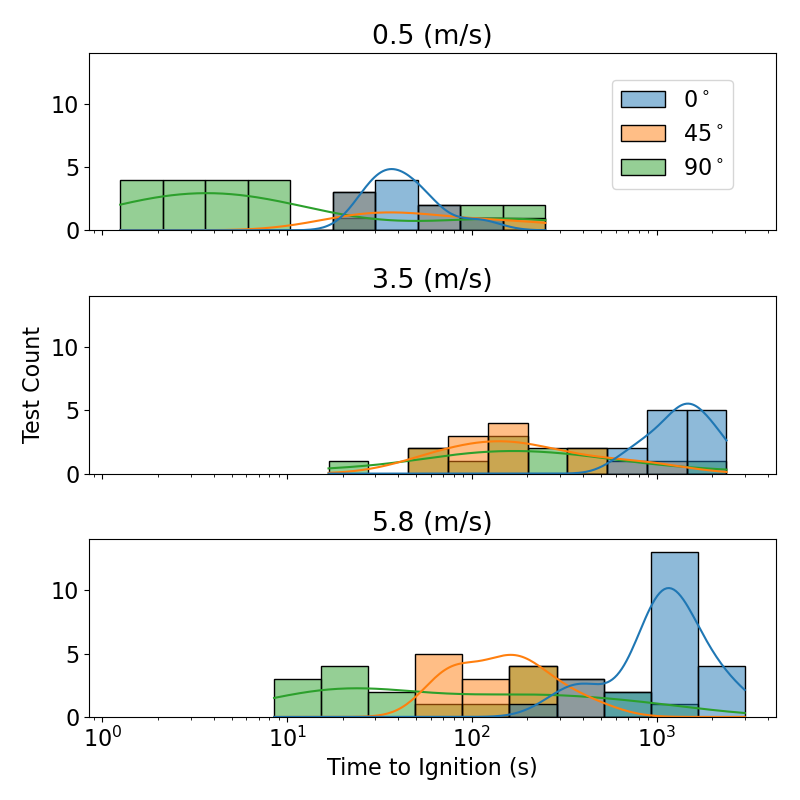
\includegraphics[width=0.5\columnwidth]{Figures/stacked_speed_hist.png}
            \caption{Histogram of time to flaming ignition for each test group. Wind speed increased from top to bottom with color indicating different heater angles.}
            \label{fig:histogramFigure}
        \end{figure}
    
    High speed images were recorded for a subset of test configurations to provide more insight into changes in ignition location resulting from changes in heater angle. Figure~\ref{fig:ignitionImages} shows images of the initial flame visible during tests of three different heater angles. A heater temperature of 450\si{\celsius} and a wind speed of 5.8\si{\meter\per\second} were used for all tests. Consistency in the location of ignition was verified by comparing images from three different ignition events for each of the heater angles. For tests where the heater was oriented at either 45\si{\degree} or perpendicular to the flow (Figure~\ref{subfig:perpendicularHeater},~\ref{subfig:45Heater}) ignition was observed to occur on the upwind side of the heater near the fuel bed. For the parallel heater orientation (Figure~\ref{subfig:parallelHeater}) ignition was observed underneath the heater in a cavity. The cavity was formed by the pyrolysis of the fuel bed. Specifically, ignition occurred at the downstream side of the cavity in the fuel bed. 
        \begin{figure}[hpbt]
             \centering
             \begin{subfigure}[b]{\columnwidth}
                 \centering
                 \begin{tikzpicture}
                 \node(a){
                 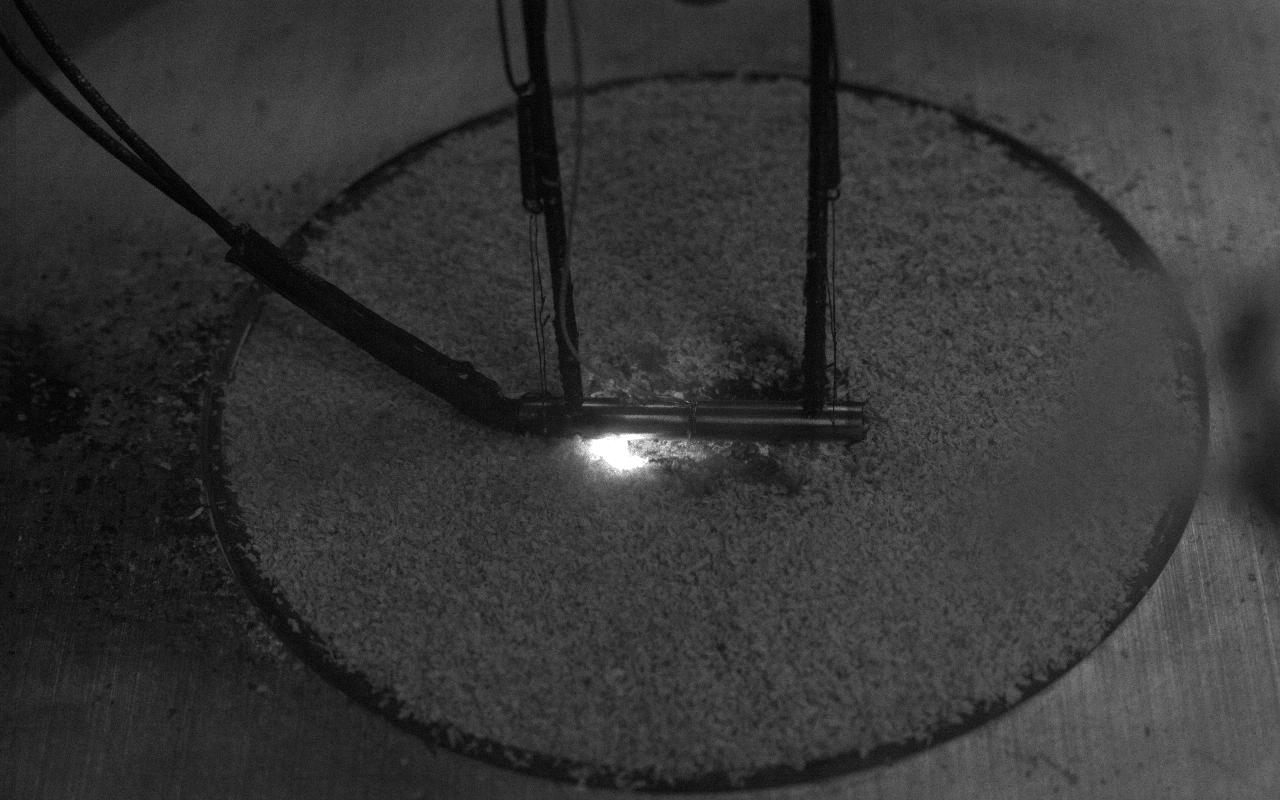
\includegraphics[width=0.75\columnwidth, trim={12cm 5cm 10cm 5cm}, clip]{Figures/5ms_0_heater_450.png}};
                 \node at(a.center)[draw, red, dashed, line width=1pt, rectangle, minimum width=65pt, minimum height=14pt,rotate=-1, yshift=-18pt, xshift=2pt]{};
                 \draw[->, thick, white] (1.5, 1.25) -- node [midway,above] {Wind Direction}(-1.2, 1.25);
                 \end{tikzpicture}
                 \caption{Parallel}
                 \label{subfig:parallelHeater}
             \end{subfigure}
             \hfill
             \begin{subfigure}[b]{\columnwidth}
                 \centering
                 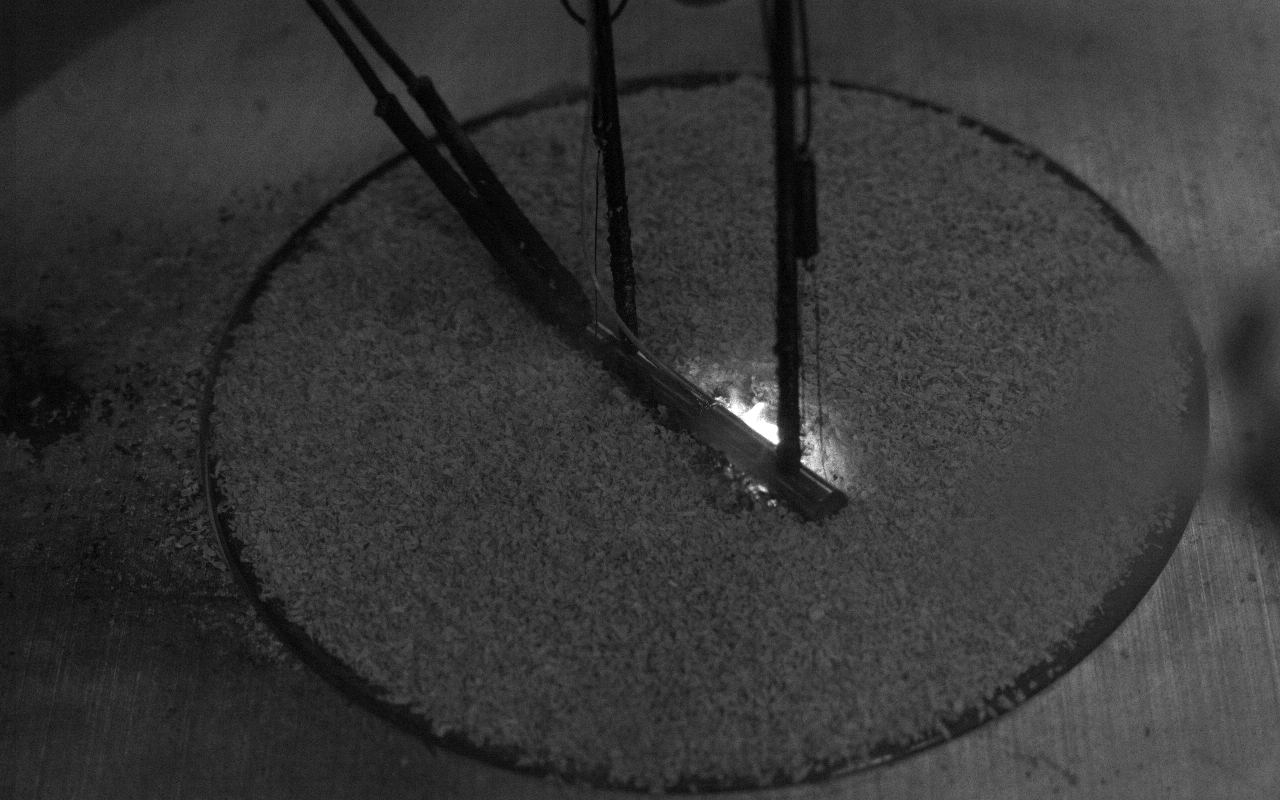
\includegraphics[width=0.75\columnwidth, trim={12cm 5cm 10cm 5cm}, clip]{Figures/5ms_45_heater_450.png}
                 \caption{45\si{\degree}}
                 \label{subfig:45Heater}
             \end{subfigure}
             \hfill
             \begin{subfigure}[b]{\columnwidth}
                 \centering
                 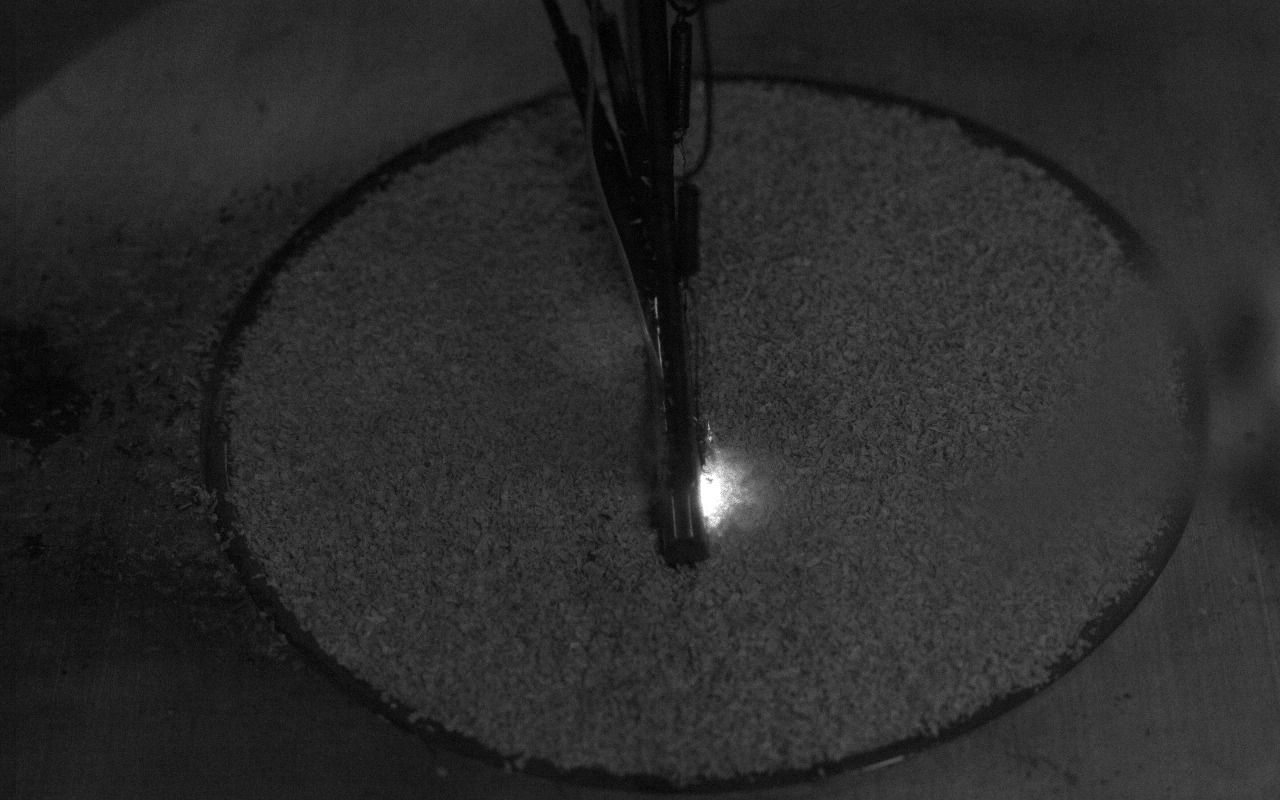
\includegraphics[width=0.75\columnwidth, trim={12cm 5cm 10cm 5cm}, clip]{Figures/5ms_90_heater_450.png}
                 \caption{Perpendicular}
                 \label{subfig:perpendicularHeater}
             \end{subfigure}
                \caption{Representative images of the location of flaming ignition for three different heater angles with a heater temperature of 450\si{\celsius} and a wind speed of 5.8\si{\meter\per\second} from right to left. The dotted rectangle in \ref{subfig:parallelHeater} highlights the cavity formed under the heater during tests.}
                \label{fig:ignitionImages}
        \end{figure}
    Differences in ignition location, and subsequent changes in ignition times, are attributed to changes in the velocity field around the heater as the orientation relative to the wind changes. As the heater is rotated from parallel to perpendicular to the flow, pyrolyzates are more likely to remain near the hottest part of the heater (approximately the center) due to the recirculation zones that form on the upwind side of the heater. When the heater is parallel to the flow pyrolyzates tend to advect away from the heater. Thus, for the perpendicular heater the recirculation zone is anticipated to have the longest pyrolyzate residence time. The pyrolyzates are also anticipated to remain near the highest temperature region of the heater. This explantion is consistent with the observation that tests where the heater is oriented perpendicular to the flow typically ignited at lower temperatures than the other orientations, as shown in Figure~\ref{fig:windSpeed}.
    
    Considering the aforementioned importance of pyrolyzate residence time on ignition enhancement, it is not immediately clear how the threshold for ignition is lowered with an increase of wind for tests where the heater is parallel to the wind direction. When the heater is positioned parallel to the flow with wind, the pyrolyzates tend to advect away from the hot regions of the heater. However, as previously noted, ignitions for the parallel case occur inside a cavity that forms underneath the heater. The fluid flow that develops with this cavity is anticipated to lead to longer residence times for pyrolyzates. The absence of a sufficient residence times until a cavity of sufficient size forms appears to be the major reason for differences in the time to ignition for the various heater orientations.
    

    Further insights into recirculation zones that form near the heater and the impact on residence times of pyrolyzates are gained from computational results. Figure~\ref{fig:CFDImages} shows streamlines passing though the pyrolysis release zones and the temperature distribution for regions where pyrolyzates are present (i.e., $\phi>$0.05) for the three heater orientations at a wind speed of 5.8\si{\meter\per\second}. The images shown in Figure~\ref{fig:CFDImages} correspond to 1\si{\second} after the release of pyrolyzates. While typical ignition times are significantly longer than 1\si{\second}, the results still provide insight into the controlling fluid mechanics. The streamlines shown in Figure~\ref{fig:CFDImages} confirm that a recirculation zone is present near the hottest region of the heater when the orientation is perpendicular or 45\si{\degree} with respect to the wind direction. The presence of recirculation zones is further supported by the presence of pyrolyzates upstream of the heater in Figures~\ref{subfig:45CFD},\ref{subfig:perpendicularCFD}.
           \begin{figure}[hpbt]
             \centering
             \begin{subfigure}[b]{\columnwidth}
                 \centering
                 \begin{tikzpicture}
                     \node{
                     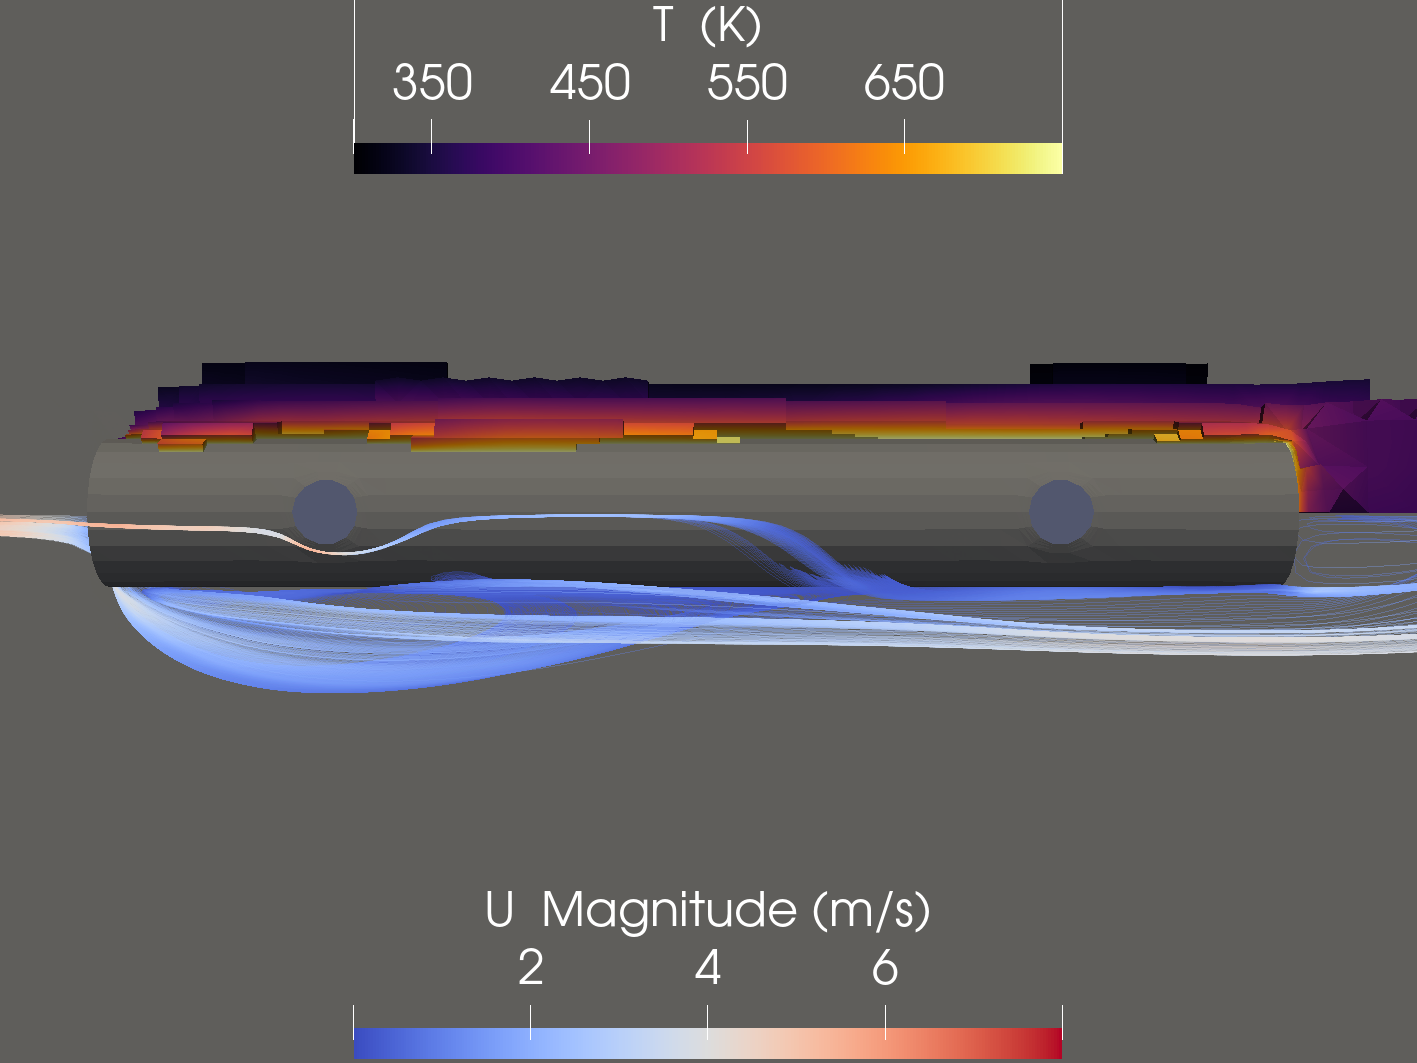
\includegraphics[width=0.45\columnwidth]{Figures/parallel_cfd_plot.png}};
                     \draw[-, dotted, very thick, red] (-2.5, 0.05) -- (2.5, 0.05);
                 \end{tikzpicture}
                 \caption{Parallel}
                 \label{subfig:parallelCFD}
             \end{subfigure}
             \hfill
             \begin{subfigure}[b]{\columnwidth}
                 \centering
                 \begin{tikzpicture}
                     \node{
                     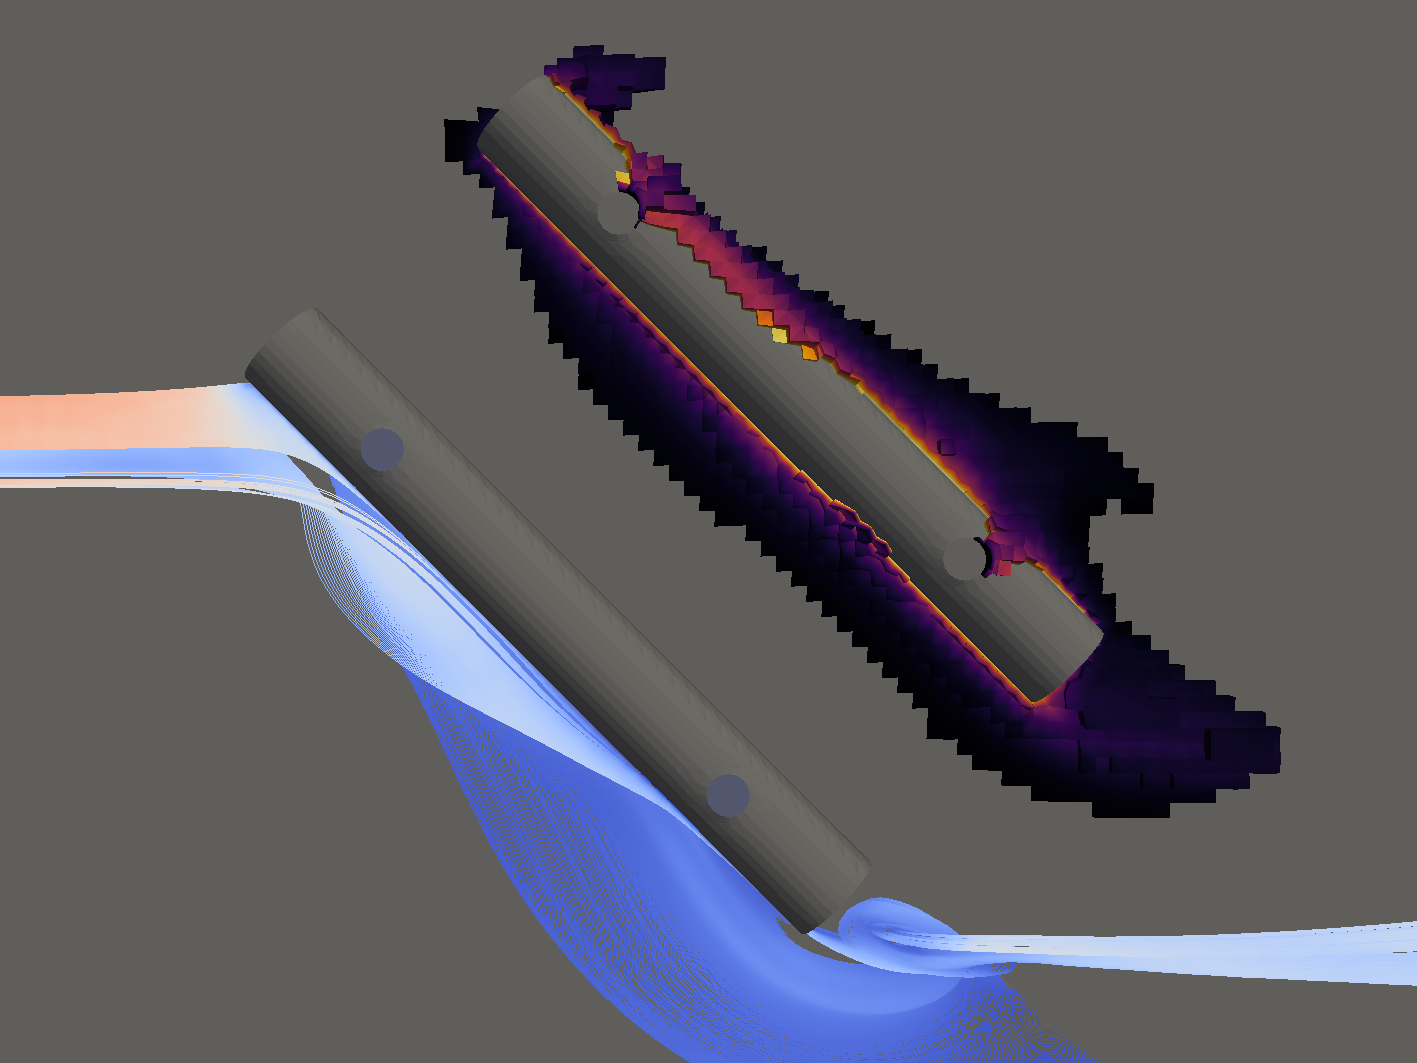
\includegraphics[width=0.45\columnwidth]{Figures/45_cfd_plot.png}};
                     \draw[-, dotted, very thick, red] (-2.1, 1.9) -- (0.9, -1.2) -- (2.5, -1.2);
                 \end{tikzpicture}
                 \caption{45\si{\degree}}
                 \label{subfig:45CFD}
             \end{subfigure}
             \hfill
             \begin{subfigure}[b]{\columnwidth}
                 \centering
                 \begin{tikzpicture}
                     \node{
                     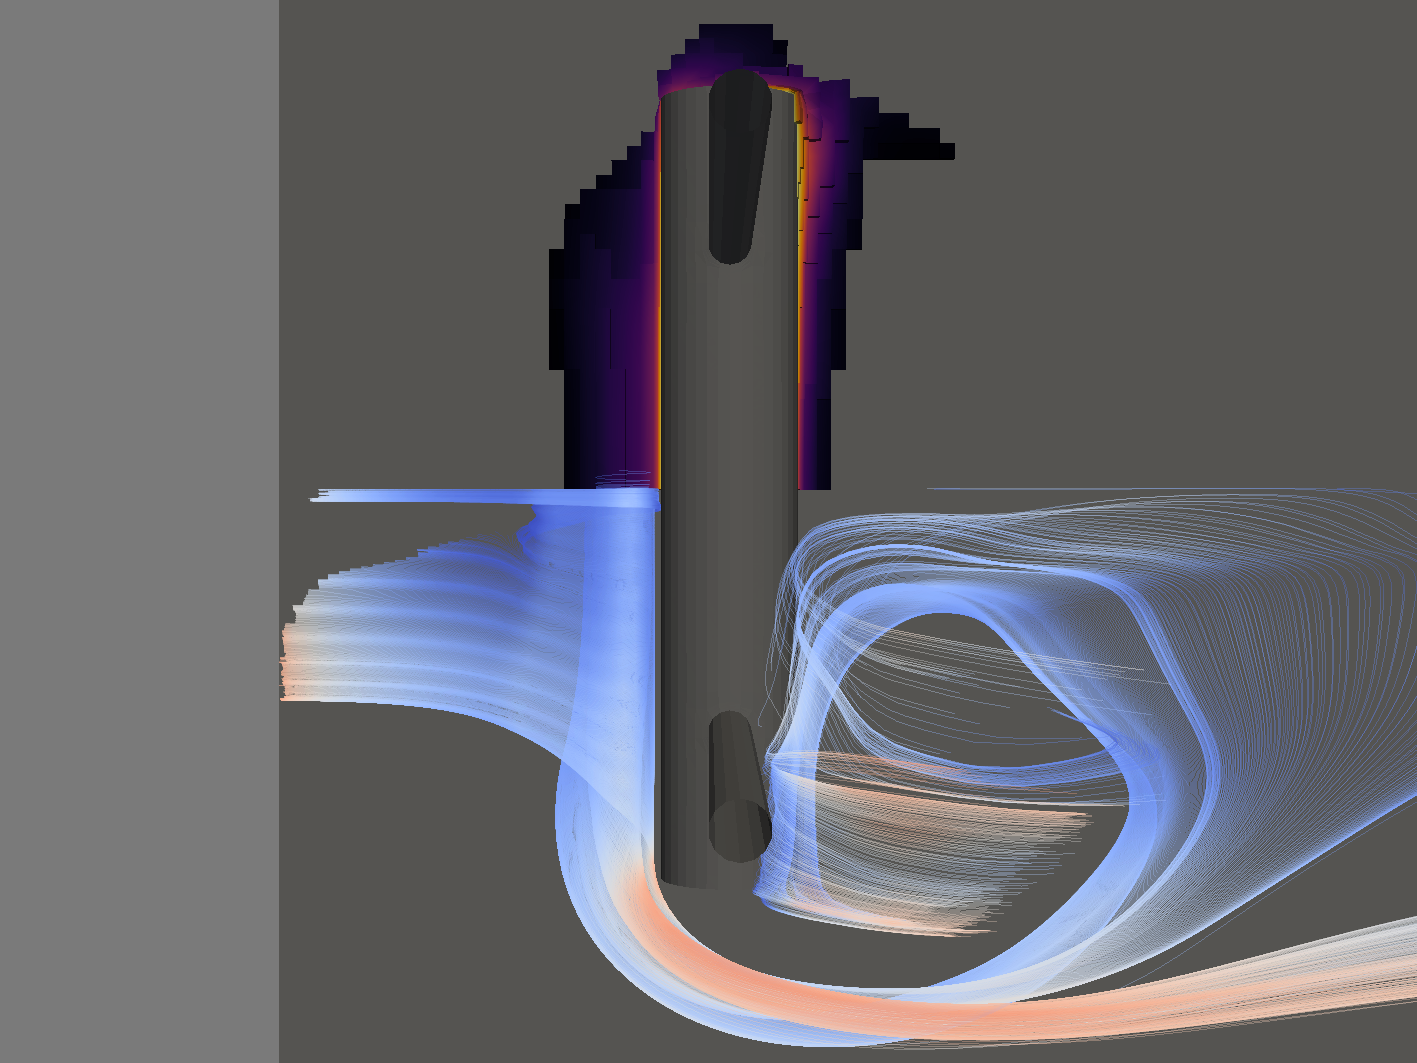
\includegraphics[width=0.45\columnwidth, trim={10cm 0cm 0cm 0cm}, clip]{Figures/90_cfd_plot.png}};
                    \draw[-, dotted, very thick, red] (-2.5, 0.18) -- (2.5, 0.18);
                 \end{tikzpicture}
                 \caption{Perpendicular}
                 \label{subfig:perpendicularCFD}
             \end{subfigure}
                \caption{CFD results showing pyrolyzate distribution and streamlines for a wind speed of 5.8\si{\meter\per\second}. The top half of each image shows the temperature distribution of pyrolyzates in regions where pyrolyzates are present (i.e., $\phi>$0.05). The bottom half of each image shows the streamlines, with the color scale representing velocity magnitude, passing through the pyrolyzate release region. Panel \ref{subfig:45CFD} shows a duplicated heater across the dotted line.}
                \label{fig:CFDImages}
        \end{figure}
    Perhaps unexpected are the characteristics of the region of the fluid anticipated to be capable of ignition ($\Phi>0.85$). For both the parallel and 45\si{\degree} heater orientation the total volume of ignitable pyrolyzates are between 4 and 6 times larger than the perpendicular heater orientation. The average temperature 3\%-5\% larger in the parallel and 45\si{\degree} heater orientations. These results suggest that the gas and temperature conditions favor ignition when the heater is not perpendicular to the flow. However, the residence time of the flammable mixture favors ignition when the heater is perpendicular to the flow. Estimates of residence time are made using the ratio of the average velocity magnitude of the pyrolysis gases with $\Phi>0.85$ and the mass release rate of the pyrolyzates from the fuel bed estimates. The average velocity of the pyrolyzates serves as a proxy for removal of combustible gases from the high temperature zone near the heater. The estimated residence time of the pyrolyzates in the perpendicular heater orientation is more than 25 times longer when compared to the parallel heater orientation and 15 times longer when compared to the 45\si{\degree} heater orientation. The differences in residence times for the three heater orientations align with those for ignition probability supporting the previous assertion that combinations of wind and geometry that facilitate long residence times ignite more readily.
    
    The correlation between time to ignition, ignition temperatures, and ignition locations indicates that ignition events are sensitive to the residence time of pyrolyzates in a high temperature zone. In other words, a firebrand is much more likely to ignite a fuel bed if the wind speed and geometry of the firebrand or firebrands promote extended residence times of pyrolyzates in a low velocity recirculation zone near the firebrand.
   
\section{Summary and Conclusions}
    Flaming ignition tests were conducted for surrogate fuel beds made of Douglas-fir particles.
    Ignition was induced by a cartridge heater, which served as a surrogate firebrand. The heater was maintained at a fixed temperature throughout each test, thus allowing sensitivities of ignition to wind speed and orientation to be further understood. The ignition probability, time to ignition, high speed imagery, and CFD results were used to quantify sensitivities to ignition related to fluid mechanics around the firebrand and fuel bed as controlled by the wind speed and heater angle. The specific conclusions of this work are as follows:
        \begin{enumerate}
            \item
            An increase in wind speed above quiescent conditions reduces the temperature required for the flaming ignition of a fuel bed. For example, an increase in wind speed of 3.5\si{\meter\per\second} from quiescent increases the ignition probability of a fuel bed from under 30\% to roughly 100\%. However, a linear increase in wind speed does not result in a linear increase in ignition probability. Thresholds in wind speed exist above which temperatures required to achieve ignition actually increase. For example, when the wind is oriented 45\si{\degree} from the heater centerline increasing the wind from quiescent to 3.5\si{\meter\per\second} reduces the temperature required for ignition probability by 30\%. However, increasing the wind speed from quiescent to 5.8\si{\meter\per\second} reduces the temperature required for ignition by only 25\%. Presumably these thresholds occur because of reductions in residence time. 
            
            \item The temperatures at which ignition occurs for porous fuel beds is sensitive to the orientation of a firebrand relative to the wind direction. Higher temperatures are typically required for ignition for a heater parallel to the flow compared to 45\si{\degree} and perpendicular to the flow. This sensitivity attributed to differences in recirculation zones and residence times of air and pyrolyzates near the hottest region of the heater. Thus, predictions of ignition probabilities that consider wind may need to include both wind speed and orientation to obtain sufficient accuracy.
            
            \item Times to flaming ignition of porous fuel beds are sensitive to the firebrand/heater angle in the presence of wind.
            The parallel heater orientation ignites at the longest time followed by the 45\si{\degree} case with the perpendicular cases igniting in the shortest amount of time. High speed images indicate that ignition typically occurrs in regions where recirculation zones occur, as shown in CFD calculations. The heightened propensity to ignition is attributed to increased residence times of pyrolyzates in the recirculation zones as supported by calculations.
        \end{enumerate}
    The conclusions of this work show that ignition is favored when a firebrand(s) land on a fuel bed under wind speeds and orientations that promote greater residence times of pyrolyzates near a high temperature region of firebrands. It was observed that increases of wind speed, of a magnitude that may commonly occur during wildfires, can increase the probability of fuel bed ignition from very unlikely to a near certainty regardless of the ember orientation to the wind. This highlights the increased risk of spot fires due to ignition of fuel beds that accompanies wind in a wildfire. 